\documentclass[11pt,oneside]{article}
\usepackage[T1]{fontenc}
\usepackage[utf8]{inputenc}
%\DeclareUnicodeCharacter{00A0}{ }
\usepackage[adobe-utopia]{mathdesign}

\usepackage{amsmath}
\usepackage[francais]{babel}
\usepackage[dvips]{graphicx}
%\usepackage{here}
\usepackage{framed}
\usepackage[normalem]{ulem}
\usepackage{fancyhdr}
\usepackage{titlesec}
\usepackage{vmargin}

\usepackage{amsmath}
\usepackage{ifthen}
\usepackage{multirow}
\usepackage{multicol} % Portions de texte en colonnes

%\usepackage{xltxtra} % Logo XeLaTeX
%\usepackage{pst-solides3d}
\usepackage{color}
%\usepackage{colortbl}
\usepackage{titletoc} % Pour la mise en forme de la table des matières

%\usepackage[crop=off]{auto-pst-pdf}
%\usepackage{bclogo}


%\usepackage{longtable}
%\usepackage{flafter}%floatants après la référence
%\usepackage{pst-solides3d}
%\usepackage{pstricks}
%\usepackage{minitoc}
%\setcounter{minitocdepth}{4}
%\usepackage{draftcopy}% "Brouillon"
%\usepackage{floatflt}
%\usepackage{psfrag}
%\usepackage{listings} % Permet d'insérer du code de programmation
%\usepackage{lmodern}
%\usepackage[adobe-utopia,uppercase=upright,greeklowercase=upright]{mathdesign}
%\usepackage{minionpro}
%\usepackage{pifont}
%\usepackage{amssymb}
%\usepackage[francais]{varioref}

\setmarginsrb{1.5cm}{1cm}{1cm}{1.5cm}{1cm}{1cm}{1cm}{1cm}

\definecolor{gris25}{gray}{0.75}
\definecolor{bleu}{RGB}{18,33,98}
\definecolor{bleuf}{RGB}{42,94,171}
\definecolor{bleuc}{RGB}{231,239,247}
\definecolor{rougef}{RGB}{185,18,27}
\definecolor{rougec}{RGB}{255,230,231}
\definecolor{vertf}{RGB}{103,126,82}
\definecolor{vertc}{RGB}{220,255,191}
\definecolor{violetf}{RGB}{112,48,160}
\definecolor{violetc}{RGB}{230,224,236}
\definecolor{jaunec}{RGB}{220,255,191}
\usepackage[final]{pdfpages} 
\usepackage[%
    pdftitle={TD Conception},
    pdfauthor={Xavier Pessoles},
    colorlinks=true,
    linkcolor=blue,
    citecolor=magenta]{hyperref}



% \makeatletter \let\ps@plain\ps@empty \makeatother
%% DEBUT DU DOCUMENT
%% =================
\sloppy
\hyphenpenalty 10000

\newcommand{\Pointilles}[1][3]{%
\multido{}{#1}{\makebox[\linewidth]{\dotfill}\\[\parskip]
}}


\begin{document}


\newboolean{prof}
\setboolean{prof}{false}
%------------- En tetes et Pieds de Pages ------------
\pagestyle{fancy}
\renewcommand{\headrulewidth}{0pt}

\fancyhead{}
\fancyhead[L]{%
\begin{minipage}[c]{1.6cm}

\includegraphics[width=2cm]{png/logo_ptsi.png}%
\end{minipage}
\rule{2cm}{.5pt}
}

\fancyhead[C]{\rule{11cm}{.5pt}}

\fancyhead[R]{%
\begin{minipage}[c]{3cm}
\begin{flushright}
\footnotesize{\textit{\textsf{Sciences Industrielles\\ pour l'Ingénieur}}}%
\end{flushright}
\end{minipage}
}

\renewcommand{\footrulewidth}{0.2pt}

\fancyfoot[C]{\footnotesize{\bfseries \thepage}}
\fancyfoot[L]{\footnotesize{2012 -- 2013} \\ X. \textsc{Pessoles}}
\ifthenelse{\boolean{prof}}{%
\fancyfoot[R]{\footnotesize{TD -- CI 4 -- Conception des mécanismes -- P}}
}{%
\fancyfoot[R]{\footnotesize{TD -- CI 4 -- Conception des mécanismes}}
}


%\begin{center}
%\textit{Centre d'intérêt}
%\end{center}


\begin{center}
 \huge\textsc{CI 4 -- Conception des mécanismes}
\end{center}


\begin{center}
 \large\textsc{Montage de Perçage}
\end{center}
\vspace{.5cm}

\begin{flushright}
\textit{D'après ressources de Jean-Pierre Pupier.}
\end{flushright}
%
%\begin{minipage}[c]{.45\linewidth}
%\begin{center}
%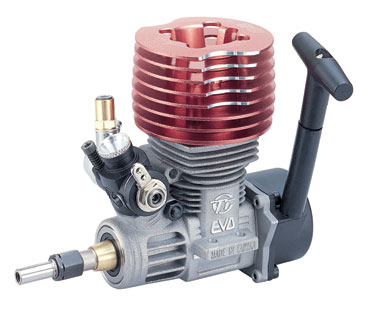
\includegraphics[height=3cm]{png/moteur}
%
%\textit{Moteur de modélisme}
%\end{center}
%\end{minipage}\hfill
%\begin{minipage}[c]{.45\linewidth}
%\begin{center}
%\includegraphics[height=4cm]{png/moteur_3D}
%
%\textit{Représentation d'un moteur de modélisme}
%\end{center}
%\end{minipage}

\begin{contexte}
\begin{itemize}
\item Objectif pédagogique : concevoir un système mécanique
\item Objectif technique : 
\begin{itemize}
\item Proposer une solution technologique permettant de concevoir un montage de perçage
\end{itemize}
\end{itemize}
\end{contexte}

\section*{Mise en situation}

Sur le montage de perçage en grande série ci-dessous, le pignon à percer $P$ est immobilisé en rotation par un doigt 3 s'engageant dans l'espace entre deux dents. Le foret peut donc percer le moyeu en respectant une position angulaire précise entre le trou percé et la denture du pignon. 

Ce doigt est guidé par une liaison glissière dans la pièce 2. Il est poussé vers le bas par un ressort pour que la position angulaire du pignon soit maintenue automatiquement lors du serrage de l'écrou 5. Lors du changement de pignon, on souhaite que 3 tienne en position relevée tout seul, ceci afin de libérer une main de l'utilisateur. Prévoyez un système qui assure cette fonction. La liaison 1/2 est un encastrement à base de pivot glissant. 



\section*{Perspectives}

\begin{minipage}[c]{.3\linewidth}
\begin{center}
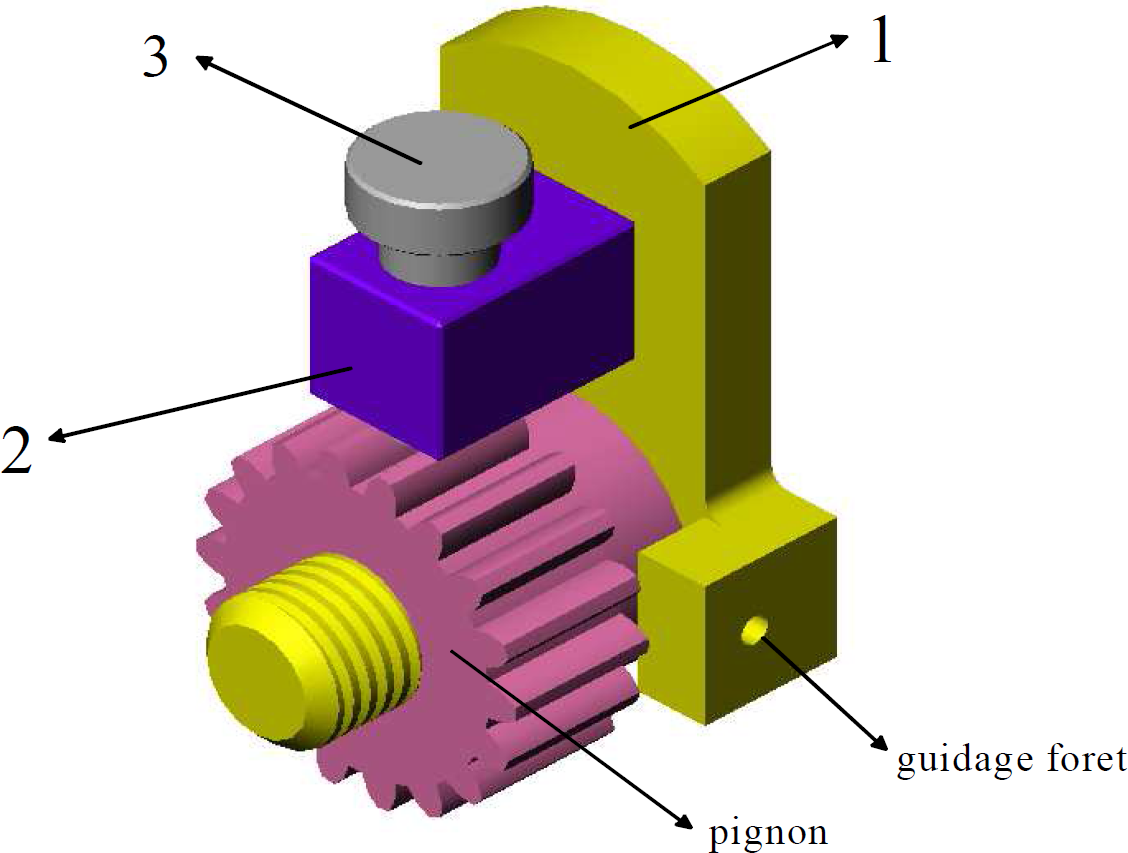
\includegraphics[height=3cm]{png/img1}
\end{center}
\end{minipage}\hfill
\begin{minipage}[c]{.3\linewidth}
\begin{center}
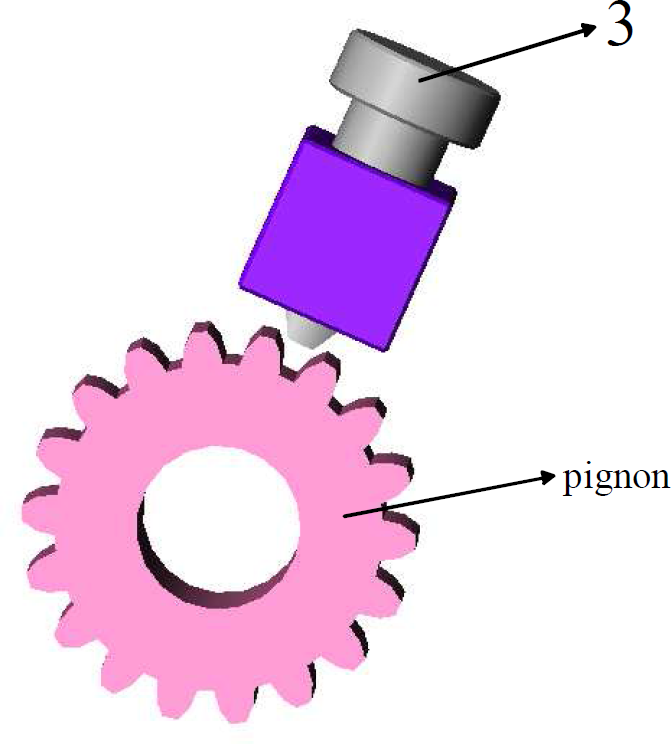
\includegraphics[height=3cm]{png/img2}
\end{center}
\end{minipage}\hfill
\begin{minipage}[c]{.3\linewidth}
\begin{center}
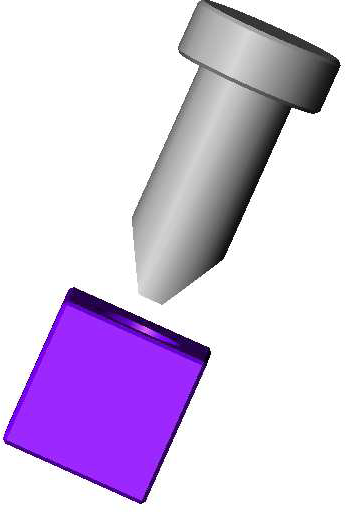
\includegraphics[height=3cm]{png/img3}
\end{center}
\end{minipage}


\section*{Schéma cinématique}


\begin{center}
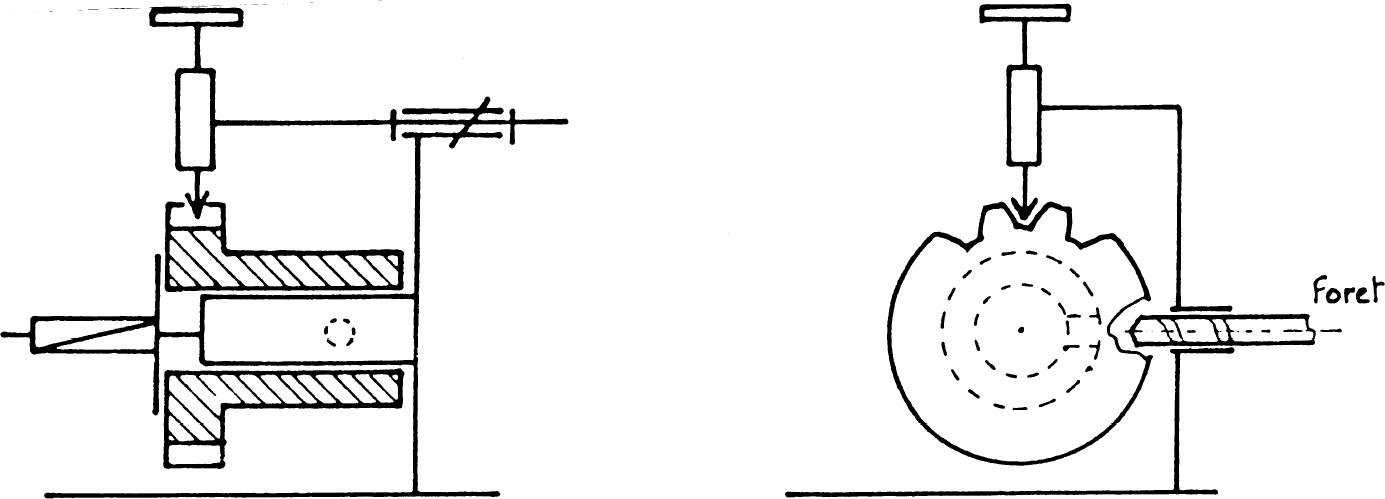
\includegraphics[width=.8\textwidth]{png/img4}
\end{center}

\section*{Travail demandé}

\paragraph*{}
\textit{Complétez le dessin de la page suivante aux instruments (le guidage de perçage ne sera pas représenté):
\begin{itemize}
\item vue de face en coupe AA
\item vue de gauche (utilisez des coupes ou des coupes partielles si nécessaires)
\item vue de dessus partielle du support 2
\end{itemize}}




\newpage 

\vspace*{\stretch{1}}

\begin{center}
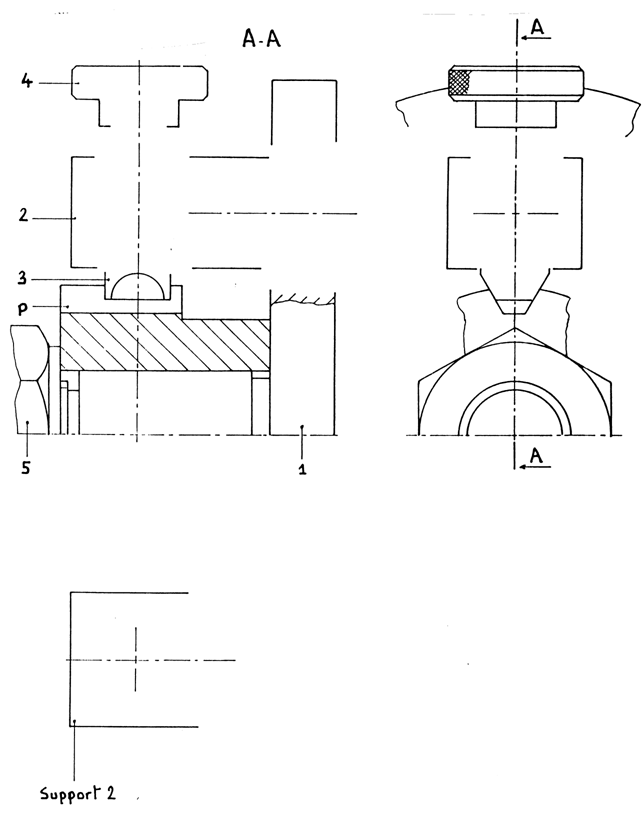
\includegraphics[width=.95\textwidth]{png/img5}
\end{center}

\vspace*{\stretch{1}}

\end{document}